% !TeX encoding = UTF-8
% !TeX program = xelatex
% !TeX spellcheck = en_US

\documentclass[master]{ustcthesis}
% doctor|master|bachelor [academic|professional] [chinese|english] [print|pdf]
% [super|numebers|authoryear]

\title{智能合约漏洞检测系统}
\author{叶家鸣}
\major{软件工程}
\supervisor{薛吟兴\ 研究员}
% \cosupervisor{钱学森\ 教授}
% \date{二〇一七年五月一日} % 注释掉则为今日
% \professionaltype{专业学位类型}
% \secretlevel{秘密}        % 绝密|机密|秘密,注释本行则不保密
% \secretyear{20}           % 保密年限

\entitle{An example of thesis template for University of Science and Technology
  of China}
\enauthor{Jiaming Ye}
\enmajor{Software Engineering}
\ensupervisor{Prof. Yinxing Xue}
% \encosupervisor{Prof. Xuesen Qian}
% \endate{May 1, 2017}      % Today if commented
% \enprofessionaltype{Professional degree type}
% \ensecretlevel{Secret}    % Top secret|Highly secret|Secret


% 加载宏包和配置
\usepackage{graphicx}
\graphicspath{{figures/}}
\usepackage{booktabs}
\usepackage{longtable}
\usepackage[ruled,linesnumbered]{algorithm2e}
\usepackage{siunitx}
\usepackage{listings}
\usepackage{color}
\usepackage{amsthm}
\usepackage{caption}
\usepackage{hyperref}
\usepackage{url}
\usepackage{float}
\usepackage{xcolor}
\usepackage{graphicx}
\usepackage{subcaption}

\lstdefinelanguage{JavaScript}{
 keywords={typeof, new, true, false, catch, function, return, null, catch, switch, var, if, in, while, do, else, case, break, contract,class, export, boolean, throw, implements, import, this, public, call, value,require},
 keywordstyle=\color{blue}\bfseries,
 ndkeywords={uint,uint256,bytes,address,mapping,memory, ERC20},
 %ndkeywordstyle=\color{pinegreen}\bfseries,
 identifierstyle=\color{black},
 sensitive=false,
 comment=[l]{//},
 morecomment=[s]{/*}{*/},
 commentstyle=\color{purple}\ttfamily,
 stringstyle=\color{red}\ttfamily,
 morestring=[b]',
 morestring=[b]"
}

\lstset{
 language=JavaScript,
 %backgroundcolor=\color{lightgray},
 extendedchars=true,
 basicstyle=\fontsize{7}{7}\selectfont\ttfamily,%\footnotesize\ttfamily,
 showstringspaces=false,
 showspaces=false,
 numbers=left,
 numbersep=0pt,
 numberstyle=\footnotesize,
 xleftmargin=2em,
 tabsize=2,
 breaklines=true,
 showtabs=false,
 captionpos=b,
 morecomment=[s][\color{red}]{**}{**}
}


\DeclareRobustCommand\cs[1]{\texttt{\char`\\#1}}
\newcommand\pkg{\textsf}

\renewcommand\vec{\symbf}
\newcommand\mat{\symbf}
\newcommand\ts{\symbfsf}
\newcommand\real{\mathbf{R}}
\newcommand{\codeff}[1]{\texttt{\footnotesize #1}}

%\newcommand{\xxx}[1]{\textcolor{red}{#1}}
%
%\newcommand{\slither}{\textsc{Slither}\xspace}
%\newcommand{\oyente}{\textsc{Oyente}\xspace}
%\newcommand{\manticore}{\textsc{Manticore}\xspace}
%\newcommand{\securify}{\textsc{Securify}\xspace}
%\newcommand{\echidna}{\textsc{Echidna}\xspace}


\begin{document}

%DOI: 10.1007/978-3-030-26574-8_6

% 研究生论文:
%   封面,原创性声明和授权使用声明
%   frontmatter: 摘要,目录,[图、表清单],[符号说明]
%   mainmatter: 正文章节,参考文献
%   appendix: 附录
%   backmatter: 致谢,已发表论文列表
%
% 本科生论文:
%   封面
%   frontmatter: 致谢,目录,摘要
%   mainmatter: 正文章节,参考文献
%   appendix: 附录

\maketitle
\makestatement

\frontmatter
% !TeX root = ../main.tex

\begin{abstract}

  \keywords{博士}
\end{abstract}

\begin{enabstract}


  \enkeywords{PhD}
\end{enabstract}

\tableofcontents
% \listoffigures
% \listoftables
%% !TeX root = ../main.tex

\begin{notation}

  \begin{notationlist}{2em}
    \item[$\displaystyle a$] The number of angels per unit area
    \item[$\displaystyle N$] The number of angels per needle point
    \item[$\displaystyle A$] The area of the needle point
    \item[$\displaystyle \sigma$] The total mass of angels per unit area
    \item[$\displaystyle m$] The mass of one angel
    \item[$\displaystyle \sum_{i=1}^n a_i$] The sum of $a_i$
  \end{notationlist}

\end{notation}



% 也可以使用 nomencl 宏包

% \printnomenclature

% \nomenclature{$\displaystyle a$}{The number of angels per unit are}
% \nomenclature{$\displaystyle N$}{The number of angels per needle point}
% \nomenclature{$\displaystyle A$}{The area of the needle point}
% \nomenclature{$\displaystyle \sigma$}{The total mass of angels per unit area}
% \nomenclature{$\displaystyle m$}{The mass of one angel}
% \nomenclature{$\displaystyle \sum_{i=1}^n a_i$}{The sum of $a_i$}


\mainmatter
% !TeX root = ../main.tex

\chapter{序言}

\section{课题研究意义及国内外现状分析}

\subsection{研究意义}
自2009年“中本聪”发布了比特币的第一篇论文以来,区块链技术受到了越来越多的关注。虽然相比传统的计算机技术,区块链技术还比较年轻,但是区块链技术本身带来的新型货币体系,包括其在各行各业的应用:去中心化的新型银行\cite{blockchain-application},基于去中心化智能合约的新型能源管理系统\cite{blockchain-in-energy}等等,无不凸显这一崭新技术在各行各业带来的革命性意义。

相比传统的中心化服务器,区块链技术的核心为去中心化的服务器系统,即网络中的每个运行区块链软件的设备都是一个独立的对等节点\cite{区块链技术及其应用研究}。相比传统的中心化服务器系统,区块链的网络中的所有节点在进行交易时不依赖于中间人,所有人都维护着同一个“账本”,并通过密码学算法对自己的交易信息进行签名加密,最后通过计算量证明来保证账本的有效和可靠性。区块链技术中体现出的去中心化,独立平等和无法随意篡改等等特性吸引了大量学者、企业、研究单位的关注。

在区块链的所有应用中,以太坊(Ethereum)是最火热的应用之一。以太坊是一个基于区块链技术的平台,发起的初衷为“建立无法被停止的应用”\cite{eth-intro}。他使用以太币(Ether)作为平台的主要货币,用密码学的算法来保证交易的正常进行。以太坊使用智能合约作为交易的主要媒介,网络中的各个节点通过智能合约完成交易、互动等功能。从2017年开始,以太坊的交易量开始高速增长\cite{eth-chart},越来越多的用户开始使用智能合约完成以太币的交易,区块链游戏的交互等等任务。

智能合约是由一种图灵完整的编程语言,Solidity,编写而成的。随着使用智能合约的人越来越多,保证智能合约使用安全的呼声也越来越高,很多学者和研究机构开始注意这门新语言,并用软件分析的方法(静态、动态分析等等)去研究这门新语言。2016年9月,一场被称为“DAO攻击”的事件窃取了价值数百万美元的以太币\cite{dao-attack}。保证以太坊软件的安全迫在眉睫。

软件分析方法,包括静态分析、动态分析、形式验证、模糊测试、代码克隆检测等等方法,是保证软件安全、分析软件特性的必经之路。以上提到的几种分析方法,各有特点,应根据使用场景进行考虑,选取合适的分析方法。其中,静态分析主要以分析软件的抽象语法树(AST),控制流图(CFG)等作为主要的分析对象,辅以特征提取\cite{deckard}、图匹配等方法,分析软件的特点;动态分析主要侧重于使用符号执行、约束求解等等方法,分析软件的特点,相比静态分析耗时更长,但准确度更高;形式验证能保证较高的软件安全等级,主要侧重于对软件流程形式化描述的分析;模糊测试的特点在于通过种子(SEED)来制作测试用例生成器,对软件的攻击面(可能存在漏洞或者缺陷的地方)输入测试用例,通过对测试用例的不断变化来达到测试软件漏洞的目的;代码克隆借助LCS(最长公共子串)算法,分析执行迹线,仿真等等方法来分析代码的相似程度。

同时,我们在从Ehterscan爬取了200万个的智能合约之后,分析统计发现,只有不到10\%的智能合约是经过验证(能找到对应源代码)的,其余智能合约以字节码(Bytecode)的形式存在于以太坊的平台上。而传统的分析方法主要以白盒分析为主,面对字节码无能为力。而这部分合约又恰好牵扯了大量的以太坊资金,如果这部分以字节码形式存在的合约的安全不能得到保证,不仅易使以太坊的用户遭受大量的经济损失,扰乱区块链的经济秩序,也会带来更多的社会不安定因素。因此,我们需要一个能直接对字节码进行分析的系统来保证这部分软件的安全。

\subsection{国内外现状分析}



\subsubsection{软件分析方法国内外现状}

目前,国内外已有大量的软件分析方法的工作。静态的分析方法通过抽象语法树(AST),控制流图(CFG),程序依赖图(PDG)等分析程序的特点。动态分析方法比如\cite{survey-dynamic}就总结了目前流行的动态分析方法,动态分析方法具有精确度高的优点,但是覆盖率和耗时长也是在使用动态方法的时候不得不考虑的问题。但更多的工作是把静态分析和动态分析结合起来,既弥补了动态分析在覆盖率上的不足,也部分解决了静态分析准确度不高的问题。
由于智能合约还属于新事物,在智能合约上的软件分析方法还以静态分析和动态分析为主,当然也有使用形式验证、模糊测试等方法分析智能合约的。静态方法包括Slither\cite{slither},是通过分析Solidity编译器生成AST,再将AST转换成IR(中间语言)和CFG(控制流图);动态方法包括Oyente\cite{oyente}、Securify\cite{securify}、Manticore\cite{manticore}都是使用了约束求解的方法分析程序的CFG,然后根据约束求解的结果来分析软件的特点,其中Oyente和Manticore均使用了在软件分析领域小有名气的约束求解器Z3\cite{z3},而Securify则使用的是Souffle\cite{souffle}进行约束求解。同样的,IBM的以太坊研究团队提出了Zeus\cite{zeus},使用了形式验证的方法实现了对Solidity软件的分析。而Echidna\cite{echidna},则是目前智能合约软件唯一的自动化模糊测试工具。智能合约虽然出生不久,但是分析智能合约的软件已经百花齐放。


\paragraph{四级节标题}

\subparagraph{五级节标题}

Lorem ipsum dolor sit amet, consectetur adipiscing elit, sed do eiusmod tempor
incididunt ut labore et dolore magna aliqua.
Ut enim ad minim veniam, quis nostrud exercitation ullamco laboris nisi ut
aliquip ex ea commodo consequat.
Duis aute irure dolor in reprehenderit in voluptate velit esse cillum dolore eu
fugiat nulla pariatur.
Excepteur sint occaecat cupidatat non proident, sunt in culpa qui officia
deserunt mollit anim id est laborum.



\section{脚注}

Lorem ipsum dolor sit amet, consectetur adipiscing elit, sed do eiusmod tempor
incididunt ut labore et dolore magna aliqua.
\footnote{Ut enim ad minim veniam, quis nostrud exercitation ullamco laboris
  nisi ut aliquip ex ea commodo consequat.
  Duis aute irure dolor in reprehenderit in voluptate velit esse cillum dolore
  eu fugiat nulla pariatur.}

% !TeX root = ../main.tex

\chapter{智能合约相关背景知识}

\section{智能合约中的常见漏洞}

智能合约有数十种漏洞,这些漏洞可以按漏洞危害,分为不同的等级。具有较高危害的几种漏洞,应该引起足够的重视。在本文中,本文参考了\cite{zeus}、\cite{oyente}、\cite{slither}等文献,提出了以下四种高危漏洞:可重入漏洞、意外异常漏洞、低级调用漏洞和自毁漏洞。本文选择这几种漏洞作为讨论的对象是因为,这几种漏洞在智能合约软件开发中较为常见,容易触发,且造成巨大伤害,在\cite{zeus}、\cite{oyente}、\cite{slither}中都对这几种漏洞提出了分析。因此,本文也必须在本文中详细研究这几种漏洞。

\subsection{可重入 (Reentrancy)漏洞}

可重入漏洞是智能合约中最负盛名的漏洞。这个漏洞源于\emph{Solidity}语言上的一个特殊机制,像\emph{JavaScript}等语言一样,\emph{Solidity}语言有回调\codeff{fallback}函数。每个合约仅能有一个回调函数,并且这种函数没有参数,没有函数名,也不会返回任何的返回值。根据\emph{Solidity}的开发文档,这种函数只会在以下两种情况被触发:当合约收到函数调用但却没有符合的函数签名(函数的唯一标识符)时;当合约接收到任何数量的以太币,即发生交易时。前一种情况极少出现,而可重入攻击抓住的就是后面的那种情况。如果一个黑客妄图发动可重入攻击,他需要做的就是在自己的合约中编写一段恶意的回调函数,从而利用回调函数的特性反复记性转账操作,达到窃取以太币的目的。另一方面来说,如果被回调函数调用的函数中不包含转账语句,可重入漏洞也可利用重复调用,来造成拒绝服务(Denial of Service)攻击。因为在以太坊的体系中,每个合约都有一定的gas限制,gas会在合约的每一次调用、任何操作中消耗掉。如果重复调用一个函数,会不断消耗被调用函数所在合约的gas,待gas耗尽,合约不能提供任何的服务,也就达到了拒绝服务攻击的目的。在2016年,黑客借助可重入漏洞对DAO合约发动攻击,共盗取了价值数百万美元的以太币。

可重入漏洞在智能合约的漏洞中算是比较灵活的漏洞,其发动攻击的方式灵活多变,目前主要的防范方式是对函数调用者的身份进行检验,新版的\emph{Solidity}编译器也对有可重入风险的函数做出了提醒,但是仍有很多已经部署在以太坊平台上的合约存在可重入的风险,因此本文很重视可重入漏洞攻击模式的的分析,并会在之后的技术开发阶段对这种漏洞进行针对性的改进。

\subsection{意外异常 (Unexpected Revert)漏洞}

意外异常漏洞是由于EVM的异常处理机制引起的一种拒绝服务 (Denial of Service) 攻击。这种漏洞多出现于在for循环中进行的批量转账操作中。产生该漏洞的主要原因是,开发者使用\codeff{require}或者\codeff{assert}去检查写于\codeff{for}循环内的转账外部调用。如果其中一次转账发生错误,\codeff{require}函数将抛出异常,并终止整个交易过程,这将导致后面的地址无法正常进行转账业务。更进一步说,如果这样的转账错误是攻击者蓄意为之,那么这个意外异常漏洞就给了攻击者一个停止当前服务的机会。\emph{Solidity}研发团队不推荐也不建议开发者们在循环中进行任何的转账业务。

如下图\ref{fig:revert_vul}代码所示,在第5行,函数试图向\codeff{refundAddress}中存放的地址发送\codeff{ether}。该函数使用\codeff{send}函数,通过不断循环进行转账。同时,该函数也针对\codeff{send}函数用\codeff{require}进行了返回值检查。如果\codeff{refundAddress}中的任何一个地址发生转账错误,则该函数将停止运行,剩下的合约地址也没法正常进行转账业务。

\begin{figure}
\begin{minipage}[htb]{1.0\linewidth}
    \begin{lstlisting}
    address[] private refundAddresses;
    mapping (address => uint) public refunds;
    function refundAll() public {
            for(uint x; x < refundAddresses.length; x++) {
                require(refundAddresses[x].send(refunds[refundAddresses[x]]));
            }
    }
    \end{lstlisting}
    %\caption{test}
\end{minipage}
\vspace{-5mm}
\caption{意外异常调用漏洞示例代码}
\label{fig:revert_vul}
\end{figure}


\subsection{低级调用 (Unchecked Low-Level-Call)漏洞}

根据\emph{Solidity}的官方文档\cite{solidity-doc},\emph{Solidity}语言中的低级调用 (call, delegatecall, etc.) 在调用失败时会返回失败布尔值,这些布尔值如果没有被用户捕捉,用户就会错过调用的失败信息,从而造成智能合约功能的混乱。\emph{Solidity}语言经过数个版本的演化,推出了相对高级的内建外部调用 (transfer, send, etc.),这些高级调用会检查调用的返回值,并在发现调用失败时抛出异常。新部署的合约使用高级的外部调用,能避免使用低级外部调用带来的低级调用漏洞。然而,由于区块链语言的特性,智能合约一经部署,无法撤除。根据本文的统计和观察,在以太坊平台上,仍有大量仍在使用的合约在使用低级调用时,对外部调用的调用结果没有任何的检查措施,这些合约有受到低级调用漏洞攻击的危险。

\subsection{自毁 (Suicidal)漏洞}

\emph{Solidity}提供内建的自毁函数\codeff{selfdestruct()},这个函数需要输入一个地址类型的参数,任何调用这个函数的合约将停止当前合约功能,并把当前合约所有的余额转移到这个参数的地址。相比直接使用\codeff{send}函数进行余额转移,使用\codeff{selfdestruct}消耗的gas\footnote{以太坊上的每条指令都有的特定属性,表示这条指令消耗的资源多少,gas为0则停止任何服务}更少。

自毁函数给智能合约提供了方便的功能,但在实际的使用中,如果自毁函数没有被很好的限制,或对调用者的身份进行严格检查,就能造成漏洞攻击。如下面\ref{fig:suicidal_vul}代码所示,\codeff{suicidal}函数实现了简单的自毁函数功能,并通过传参来确定转移余额的目标地址。可是,函数的访问是公开的,任何一个访问该合约的用户都能调用这个自毁函数,并把自己的攻击地址作为余额的转账地址,造成自毁漏洞攻击。\emph{Solidity}研发团队在开发文档中提醒开发者要限制自毁函数的调用,并对调用者进行身份检查。

\begin{figure}
\begin{minipage}[htb]{1.0\linewidth}
    \begin{lstlisting}
    contract gamble{
        ...
        public suicidal(address target) public {
            selfdestruct(target);
        }
    }
    \end{lstlisting}
    %\caption{test}
\end{minipage}
\vspace{-5mm}
\caption{自毁漏洞示例代码}
\label{fig:suicidal_vul}
\end{figure}


\section{前沿智能合约分析工具}

\subsection{静态分析工具}

\subsubsection{传统静态分析工具}

传统静态分析是借助程序的中间语言(IR)、抽象语法树(AST)、控制流图(CFG)等等工具去分析程序特点的分析方法。静态分析方法的主要特点是覆盖率高(即能保证覆盖程序的尽可能多的执行路径),但准确率低。现有的传统静态分析工具代表如Slither\cite{slither},他的分析路径如下图\ref{fig:slither_proccess}所示:

\begin{figure}[h]
\vspace{+2mm}
  \centering
  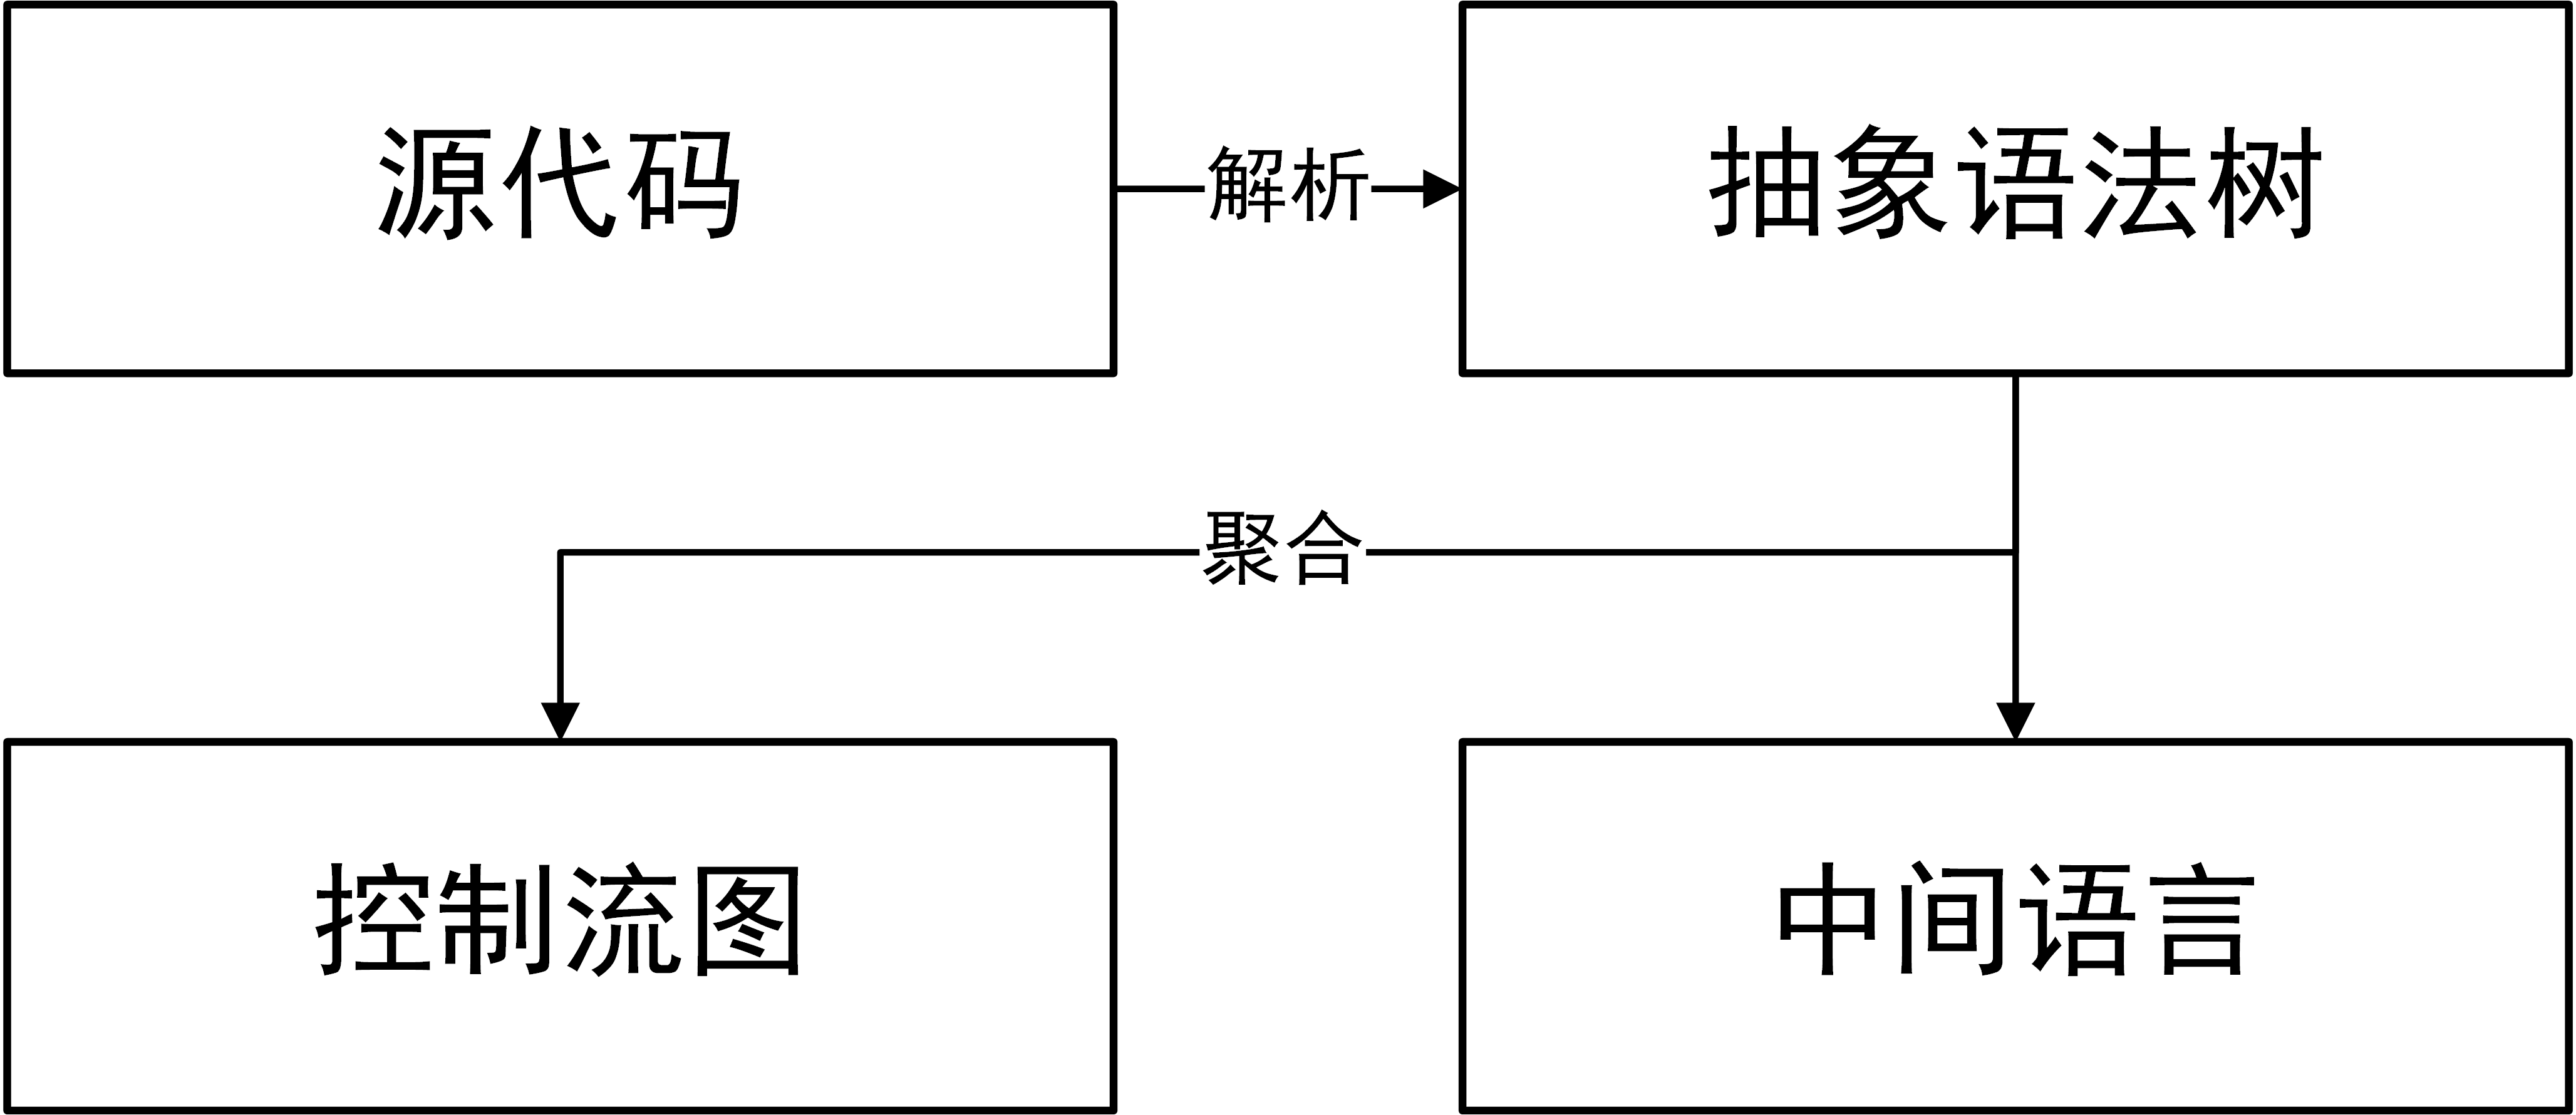
\includegraphics[width=0.55\textwidth]{figures/slither_process.png}
  \caption{\textsc{Slither}系统流程图}
  \vspace{-5mm}
  \label{fig:slither_proccess}
\end{figure}

以源代码作为输入,\textsc{Slither}首先借助\emph{Solidity}编译器将源代码经过编译,获取了程序的抽象语法树,再在AST上通过聚合、规则匹配的方式生成Slith中间语言(Intermediate Representation)和控制流图(Control Flow Graph)。由于\emph{Solidity}编译器生成了结构性强的抽象语法树(Abstract Syntax Tree),为分析提供了方便,故Slither能够在AST上如此顺利地实现IR和CFG的转换。其中,Slith IR是\textsc{Slither}的开发团队设计的一款中间语言,对源代码的常见操作做了不同程度的抽象。在以上所有步骤都完成之后,\textsc{Slither}再借助不同的探测器对生成的CFG进行探测。探测器中是\textsc{Slither}预先设定好的探测规则,如果在分析过程中发现和探测规则吻合的程序片段,探测器就会报告这个程序片段存在漏洞。故严格意义上来说,\textsc{Slither}是一款基于规则的漏洞检测软件。一方面来说,基于规则的设定提升了\textsc{Slither}的检测速度,也保证了它的可扩展性;另一方面,如果规则的制订不够合理,或者规则的分析程度不能做到抽象性和准确性的平衡,基于规则的检测方法就会带来很高的假正确率(False Positive Rate)。例如,\textsc{Slither}中针对可重入漏洞的检测规则如下图\ref{fig:slither_reentrancy_flow}所示:

\begin{figure}
\vspace{+2mm}
  \centering
  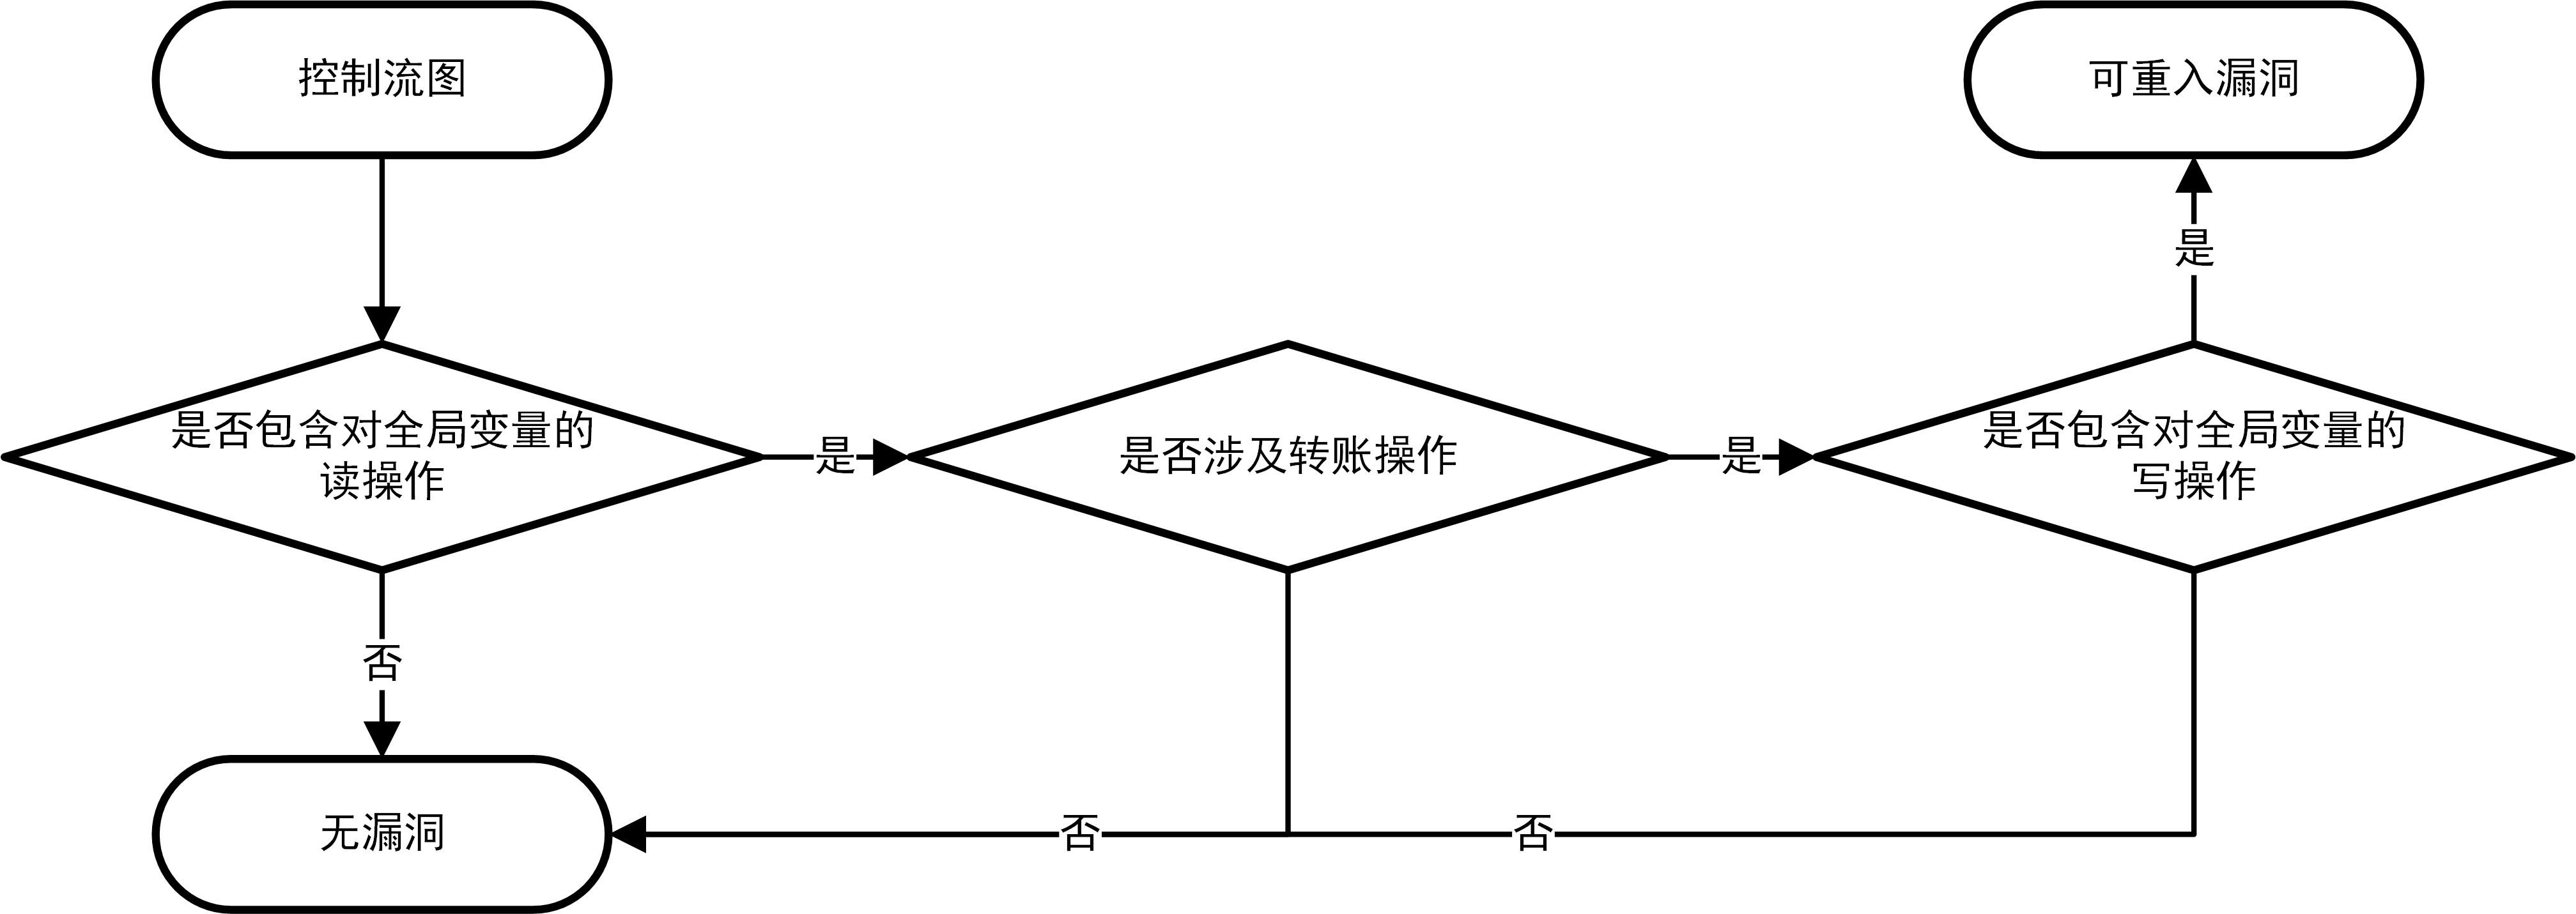
\includegraphics[width=0.9\textwidth]{figures/slither_reentrancy_flow.png}
  \caption{\textsc{Slihter}对可重入漏洞的判断逻辑}
  \label{fig:slither_reentrancy_flow}
\vspace{-5mm}
\end{figure}

在这个检测规则中,检测器逐一扫描CFG中的各个代码块,如果规则符合,就会报告漏洞。可重入漏洞的规则主要由三部分组成,其中任何一个条件不满足,都会被判断为清白的代码块,这三个条件包括:是否有对全局变量的读取操作、是否涉及交易过程、是否有对全局变量的写入操作。这个规则对可重入漏洞中的某一类型做出了准确地判断,但对其他新型变种可重入攻击,这个规则显得不够灵活。规则的修订过程是无止境的,基于规则的探测器不能保证漏洞检测的鲁棒性。如图\ref{fig:reentrancy_variant}所示,在这种潜在的可重入漏洞中,在安全的交易操作后面紧跟了一个危险的外部调用,这个危险的外部函数调用能触发对当前函数的二次访问。在本文看来,即使只重入了一次,只要造成经济损失,就要算作可重入漏洞。在本文观察\textsc{Slither}的内部原理后,本文发现\textsc{Slither}会漏掉类似的漏洞代码,它在安全的交易操作之后,没有发现对全局变量的写操作,这和\textsc{Slither}的检测规则相悖,故停止了检查,从而漏洞了紧随其后的危险外部调用。类似的例子还有很多,对于基于规则匹配的静态分析技术而言,不断修缮规则是一项长期的工作。

\begin{figure}
\vspace{+2mm}
  \centering
  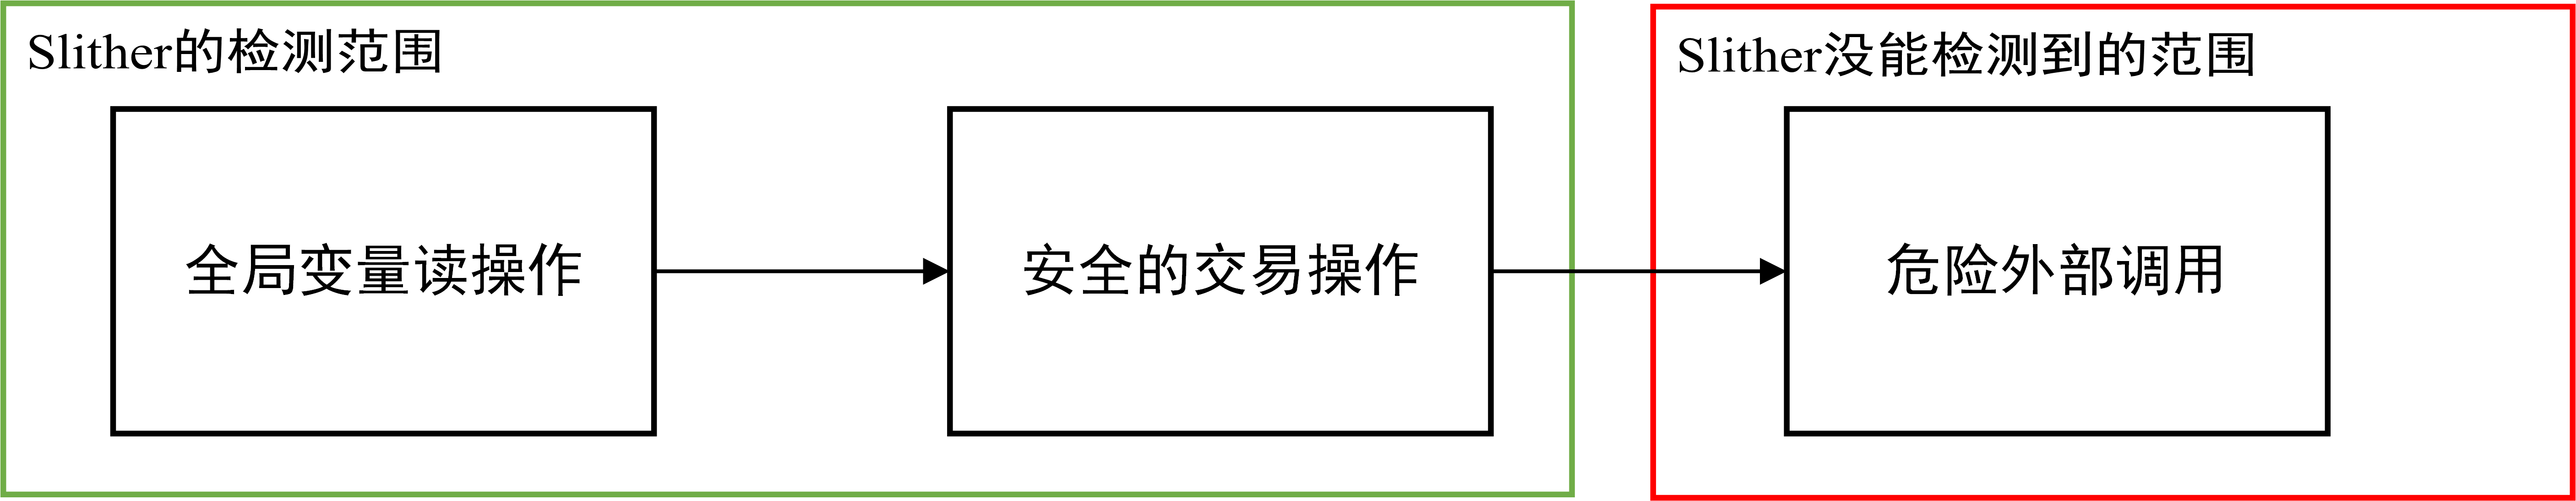
\includegraphics[width=0.9\textwidth]{figures/variant_reentrancy_pattern.png}
  \caption{\textsc{Slither}漏掉的潜在可重入漏洞}
  \label{fig:reentrancy_variant}
\vspace{-5mm}
\end{figure}



\subsubsection{符号执行分析工具}

符号执行分析工具主要将变量用符号进行标识,并利用约束求解器进行求解,来达到测试软件的墓地。符号执行工具没有像动态分析工具那样使用真实的用例观察软件的运行情况,而是利用约束求解技术或者其他技术代替真实值执行。在智能合约领域,代表的符号执行分析工具有\textsc{Oyente}\cite{oyente},\textsc{Oyente}的分析过程如下图\ref{fig:oyente_process}所示:

\begin{figure}
\vspace{+2mm}
  \centering
  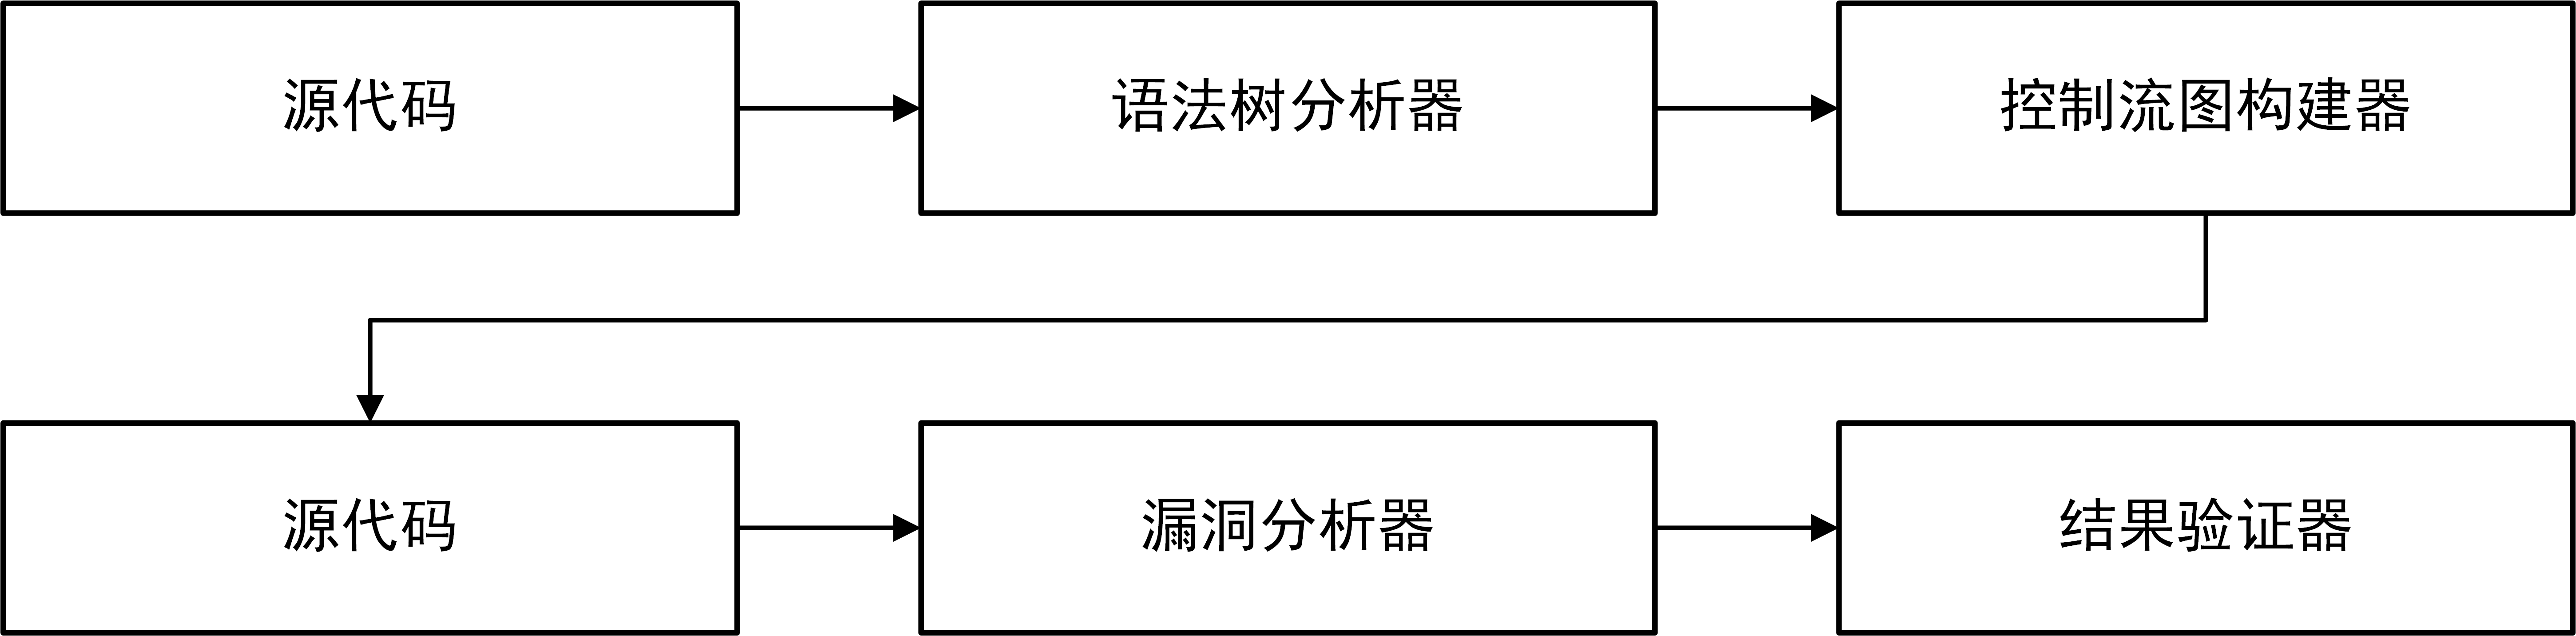
\includegraphics[width=0.9\textwidth]{figures/oyente_process.png}
  \caption{\textsc{Oyente}系统流程图}
  \label{fig:oyente_process}
\vspace{-5mm}
\end{figure}

\textsc{Oyente}的输入为源代码,再借助\emph{Solidity}编译器生成AST,进而生成CFG,再在CFG的基础上用Z3约束求解器进行符号执行,最后分析约束求解器的返回值并根据输出报告。\textsc{Oyente}的探测器在分析约束求解器的结果时,也用了基于规则的方法,如果约束求解器的结果和规则相符,则证明这个程序片段是有可能存在漏洞的。在执行流程的最后还有个验证器负责减少程序的误判。

作为典型的符号执行分析工具,\textsc{Oyente}充分体现了他的特点,它在同样的数据集上花费了近十倍于\textsc{Slither}的分析时间,耗时较长。遗憾的是,\textsc{Oyente}的结果并不是很好,输出的结果有很高的假正确率,本文推测是由于规则设置的不合理导致的。但不可否认的是,\textsc{Oyente}作为静态分析工具,能够分析一些传统静态分析工具无法分析的漏洞,比如整数的上溢、下溢,栈溢出等等,这些漏洞无法通过传统分析方法得出。

其他的分析工具如\textsc{Manticore}\cite{manticore},也采用了符号执行分析技术,这种技术带来了更高的精确度的同时也容易引入更差的性能表现。

\subsection{动态分析工具}

动态分析工具主要依赖于动态分析技术进行分析,这种技术使用测试用例作为输入,观察软件运行的状态(内存,耗时等等)和输出结果,进行分析并寻找程序漏洞。早期的动态分析技术多为黑盒测试,使用测试用例生成器不断产生测试用例,输入到软件中并观察结果。黑盒测试不依赖于软件本身的结构信息,只分析软件的运行状态及输入和输出之间的关系。早期的测试用例也是根据程序员本身的领域知识随机产生,由此也带来了测试用例测试效率低的问题——产生了大量的测试用例,却无法有效地测试到漏洞。为了解决以上问题,灰盒测试以及模糊测试诞生了。灰盒测试借助了静态分析技术来提高性能和表现,而模糊测试通过不同的标准来限制测试用例的数量,追求用最少的测试用例达到最高的测试效果。传统的模糊测试主要以程序的覆盖率作为标准,来引导整个测试过程,并采用了基于模型的或基于突变的测试用例生成器,解决了黑盒测试的主要问题,提高了测试效率。

在\emph{Solidity}这门语言上,静态分析工具有一定的局限性。例如,对于复杂的控制流关系,静态分析技术无法保证漏洞的触发问题,即虽然静态技术能保证很高的路径覆盖率,却不能保证检测到的漏洞能触发。\emph{Solidity}语言实现的智能合约,多数功能简单,控制流图相比传统的Linux软件要小很多,但即使在这样的软件上,静态分析也不能打到完美的效果。为此,在某些场景下,需要结合动态分析技术进行分析。当下前沿的动态分析工具有\textsc{ContractFuzzer}\cite{contractfuzzer},\textsc{ContractFuzzer}对\emph{Solidity}字节码进行测试,以函数的覆盖率为引导生成测试用例,并修改了底层EVM虚拟机以提供更多信息,综合以上信息进行漏洞的分析。虽然以函数的覆盖率为引导的测试在智能合约软件上可能效果不太好,但是不可否认\textsc{ContractFuzzer}迈出了重要的一步。同样的模糊测试工具还有\textsc{Echidna}\cite{echidna},它是基于Haskell进行开发的,提供对\emph{Solidity}函数的测试功能。但\textsc{Echidna}需要手工对\emph{Solidity}的函数进行打桩,这意味着它的扩展性有限,在面对大数据集时可能会耗费大量时间。

\subsection{其他分析工具}

还有其他类型的程序分析工具比如基于形式验证的工具。形式验证是一种高级的软件安全分析技术,它直接分析软件的形式化描述,而不是软件的源代码,并使用数学工具证明软件的安全。形式验证往往能保证较高的安全等级,在一些有很高安全等级需求的软件,如果空客公司的飞行管理软件,需要形式验证来保证软件的安全。

在\emph{Solidity}上,有形式化验证的分析工具\textsc{Zeus}\cite{zeus},但是\textsc{Zeus}的团队在投递论文之后并没有公开程序源代码,也没有试图将工具商业化,因此本文没办法观察\textsc{Zeus}的运行原理。

\subsection{现有智能合约分析工具总结}

本文收集了当前公开了信息的\emph{Solidity}分析工具的资料,并在表\ref{tab:all_tools}中做出总结:

\begin{table}[h]
    \centering
    \caption{\emph{Solidity}前沿检测分析工具汇总}
    \small
    \begin{tabular}{ccccc}
\toprule
 Tool Name & Github Stars & Open Sourced & Method & Technique \\
 \midrule
 \textsc{Mythril}\cite{mythril} & 1177 & $\checkmark$ & Dynamic & Constraint Solving \\
 \textsc{MythX}\cite{mythx} & n.a.& $\times$ & Dynamic & Constraint Solving    \\
 \textsc{Slither}\cite{slither} & 247 & $\checkmark$ & Static & CFG Analysis   \\
 \textsc{Echidna}\cite{echidna} & 306 & $\checkmark$ & Dynamic & Fuzzy Testing  \\
 \textsc{Manticore}\cite{manticore} & 1546 & $\checkmark$ & Dynamic & Testing  \\
 \textsc{Oyente}\cite{oyente} & 663 & $\checkmark$ &  Static & Symbolic Analysis   \\
 \textsc{Securify}\cite{securify} & 129 & $\checkmark$ &  Static & Datalog Analysis   \\
 \textsc{SmartCheck}\cite{smartcheck} & 47 & $\checkmark$ & Static & AST Analysis  \\
 \textsc{Octopus}\cite{octopus} & 153 & $\checkmark$ & Static & Reverse Analysis  \\
 \textsc{Zeus}\cite{zeus} & n.a. & $\times$ & Static & Formal Verification   \\
 \textsc{ContractFuzzer}\cite{contractfuzzer} & 34 & $\checkmark$ & Dynamic & Fuzzy Testing  \\
 \bottomrule
\end{tabular}
\label{tab:all_tools}
\end{table}

从表中可以看出,大部分工具现有的检测工具都选择了开源。MythX选择了商业化,对软件后续的更新进行了闭源处理;Zeus在2018发表于NDSS,文章中Zeus具有着卓越的效果,但在发表文章之后,Zeus的开发团队并没有把Zeus开源的想法。在现在的这篇工作中,本文无法接触到这两种工具,无法从内部剖析他们检测漏洞的原理和规则,因此本文只能讨论现有的开源工具。有趣的是,在现有的检测工具中,采用静态检测方法的工具和采用动态检测方法的工具各占一半,静态工具速度快,但动态工具的检测准确度高,两个类型的工具互相结合,才能有更好的检测效果。

\section{智能合约字节码相关知识}

字节码是一种经过\emph{Solidity}编译后生成的十六进制代码串,能直接被EVM运行。字节码中的那部分字节都可以和特定的操作对应起来。如表\ref{tab:opcode_gas}所示:

\begin{table}
  \centering\small
  \caption{操作码gas消耗对应表}
    \begin{tabular}{cccc}
      \toprule
      % after \\: \hline or \cline{col1-col2} \cline{col3-col4} ...
      Opcode & Name & Description & Gas \\
      \midrule
      0x00 & STOP & Halts execution & 0 \\
      0x01 & ADD & Addition operation & 3 \\
      0x02 & MUL & Multiplication operation & 5 \\
      0x03 & SUB & Subtraction operation & 3 \\
      ... & ... & ... & ... \\
      \bottomrule
    \end{tabular}
  \label{tab:opcode_gas}
\end{table}

操作名和字节码中的十六进制码一一对应,每个操作都有特定的意义,并且有着不同的gas消耗量。因此,本文分析字节码的第一步应该从对应表着手,先将十六进制码转换成对应的操作名,区分出操作码和操作数,并将字节码翻译为汇编码。

仅仅将十六进制码转换为汇编码是远远不够的。在学习相关文献和黄皮书后,本文对\emph{Solidity}字节码的结构有了更深刻的认识。\emph{Solidity}将源代码编译后,会生成构造函数(Creation Function)和运行时函数(Runtime Function)两部分。这两部分中,有大量代码和源代码没有关系,是EVM为了更好的运行在编译时加上的。

一个完整的构造函数,除了构造器本体,还包括重置内存指针(Free Memory Pointer)、支付检查(Non-payable Check)、构造器参数获取(Retrieve Constructor Parameters)、拷贝运行时函数地址(Copy Runtime Function Address)等等部分。这些代码除了构造器本体外,其余的部分都是和源代码无关的代码,因此本文在反编译字节码时,可以考虑去掉相关代码,考虑到这些代码在大多数情况下不会有太多变化,这个环节的实现难度适中。
运行时函数包括了源代码的主体部分,体量也比构造函数大不少。在运行时函数的开始部分,会先重置内存指针、支付检查,随后会将调用的函数名称传入函数选择器。函数选择器中存放了源代码中各个函数的函数签名,将传入的函数名称经过hash和函数签名进行比对,就可以得到各个函数在内存中的位置。在获取函数位置之后,并不能马上直接运行函数主体,EVM会先运行函数包装器(Function Wrapper)中的内容。包装器的主要功能包括保管函数入口地址、清理内存、接受函数返回值等等,它的存在保证了函数的正常稳定运行。在包装器准备好之后,才会进入函数的主体部分。主体部分包括了源代码中的绝大部分内容,故在反编译过程中,如果能跳过函数选择器和函数包装器,直接找到函数的主体部分,将会大大减少本文的分析代码量。

此时汇编码还没有结束,在汇编码的最后部分是大量的无效代码,这部分的十六进制代码无法和对应表中的任何操作联系起来。事实上,这部分的代码并不是真的无效代码,这部分的代码称为元数据hash(Metadata Hash)。根据黄皮书介绍,每个合约部署在区块上时,会根据合约的信息(函数签名、构造器参数、函数数量等等)生成一个hash值,每个合约的hash值都是唯一的,这个hash值称之为元数据hash,放在运行时函数的最后部分,作为合约的指纹小心存放。在构造函数和运行时函数中并不会有任何的函数调用会涉及这一部分的代码,它们仅作为合约的唯一代码在部署时被使用。

% !TeX root = ../main.tex

\chapter{主要研究方法及技术路线}

\section{现有工具漏洞检测能力}

在开始进行实验之前,我们需要对现有工具的检测能力进行充分地调研。只有在了解现有工具的检测能力、检测特点的情况下,我们才能开始进行漏洞标准库的构建和新工具的研发工作。为此,我们调研了当下对Solidity的研究工作,有的工作来自于商业团队,有的来自于学术团队;有的工具已经开源,并具备一定的社区影响力,有的工具发表于计算机顶级国际会议,带来了巨大的科研价值。发表于国际会议的工作,有的没有开源,对于这些没有开源的工作,虽然有论文做详细的说明,但由于不能获取到源代码,我们没办法对系统的内核做更深一步的分析,所以这些工具尽管有一定的学术影响力,我们也只能放弃。对于已经开源的工作,有些工具的开发逻辑不够严谨,或者相关文档不够完备,这些工具我们虽然能取得它们的源代码,但由于无法清晰地分析系统实现,故这些工具我们也无法很好地去分析他们的检测原理和检测能力。综上,在经过我们的筛选后,我们对如下工具在主要漏洞上的检测能力做出了总结,并和我们的系统\textsc{Athena}做比较列于表\ref{tab:detection_capability}。

\begin{table}
  \centering\small
  \caption{现有工具对于主要漏洞的检测能力总结}
  \begin{tabular}{cccccc}
    \toprule
    % after \\: \hline or \cline{col1-col2} \cline{col3-col4} ...
     & \textsc{Slither} & \textsc{Oyente} & \textsc{Smartcheck} & \textsc{Securify} & \textsc{Athena} \\
     \midrule
    可重入漏洞 & $\checkmark$ & $\checkmark$ & $\times$ & $\checkmark$ & $\checkmark$ \\
    意外异常漏洞 & $\checkmark$ & $\times$ & $\checkmark$ & $\times$ & $\checkmark$ \\
    低级调用漏洞 & $\checkmark$ & $\times$ & $\checkmark$ & $\times$ & $\checkmark$ \\
    自毁漏洞 & $\checkmark$ & $\times$ & $\times$ & $\times$ & $\checkmark$ \\
    \bottomrule
  \end{tabular}
  \label{tab:detection_capability}
\end{table}

上表所列的工具皆为静态分析工具,其中\textsc{Oyente}主要使用符号执行分析技术;\textsc{Securify}主要把代码转换成Datalog语言,并使用\textsc{Souffle}进行分析。\textsc{Slither}和\textsc{Smartcheck}采用的是传统的静态分析技术,即通过分析源代码得到程序的控制流图,并在控制流图上用预先设定好的匹配规则去寻找漏洞。从表中不难看出,使用传统静态分析技术的工具分析能力都比较不错,\textsc{Slither}支持我们提及的所有漏洞的检测,\textsc{Smartcheck}不支持两个漏洞的检测;而使用符号执行分析技术,包括使用其他静态分析技术的工具,对主要漏洞的支持都不太好,甚至只支持一个漏洞的检测。值得一提的是,这两个工具\textsc{Oyente}和\textsc{Securify}皆是在源代码编译之后产生的字节码上进行软件分析的,字节码的分析提供的信息更少,相比之下\textsc{Slither}和\textsc{Smartcheck}都是对源代码或者中间语言进行分析,故我们推测是由于技术路线的差异造成它们在不同漏洞上的分析难度不同,也就没办法支持所有漏洞的分析任务。

\section{使用克隆分析技术寻找漏洞代码}

在克隆代码分析技术中,按照代码相似的不同程度,我们可以把代码划分为以下几种克隆层次:
\begin{itemize}
  \item \textbf{第一类克隆:完全克隆。}这种克隆下层次下的相似代码之间完全相似,没有任何差异。
  \item \textbf{第二类克隆:重命名克隆。}这种克隆层次下的代码之间绝大部分相似,在类型、标识符、注释、空格之间有些许差异。
  \item \textbf{第三类克隆:重构克隆。}这种克隆层次下的相似代码之间具有结构层次的不同,例如缺少部分语句,多出部分语句,语句顺序不同等等。
  \item \textbf{第四类克隆:语义克隆。}这种克隆层次下的相似代码之间可能完全不同,但他们具有相同的语义,实现了相同的功能或流程。
\end{itemize}
从克隆层次的分类我们可以看出,第一类克隆和第二类克隆不涉及代码结构上的变化,因而能用比较简单的技术进行分析。在Kamiya等人的工作中\cite{ccfinder},使用了基于标记的克隆分析技术来寻找克隆代码,将代码的关键部分转换为标记,再在标记上进行分析寻找。由于前两类克隆代码的分析并没有什么挑战,因此现在已经有很多这方面的工作。对于第三类克隆,因为代码之间出现了语句结构的差异,例如多的语句,少的语句等等,直接借助基于标记的克隆分析技术来寻找克隆代码可能会遇上很多困难。为了解决这一问题,有人提出了提取代码特征转换成特征向量,并在高维空间进行比较的办法\cite{deckard},也有的工作提出使用软件的控制流图进行语句结构的比较\textcolor{red}{Add citation here}。而对于第四类克隆的分析,仍然是当前软件工程学界的一个有挑战的课题。有的工作提出使用深度学习算法进行代码语义的提取\textcolor{red}{Add ICST citation},但仍有很大的局限性如学习算法的数据集匮乏,很难找到数量充足且质量上乘的训练材料。因此,在讨论克隆分析技术时,我们主要解决的是寻找前三类克隆的相似代码的问题。

针对以上三种代码克隆等级,之前的工作提出了很多不同粒度的解决方案:
\begin{enumerate}
  \item \textbf{基于标记粒度的克隆分析技术:}使用基于标记力度的克隆分析技术试图使用将代码语句转换成标记序列,然后再在标记序列上比较相似度。这其中最出名的工作有CP-Miner\cite{cpminer}。CP-Miner解析了程序代码,并使用了“最频繁子序列挖掘”算法对代码生成的标记序列进行比较。这个算法由CloSpan\cite{clospan}这篇工作提出。多亏了CloSpan这篇工作在改进算法运行效率方面的贡献,CP-Miner可以在大规模代码,如Linux内核代码下仍保持了较低的内存占用。但是,CP-Miner的运行时间复杂度在最坏情况下为$\mathcal{O}(n^{2})$,$n$为代码行数,运行耗时较长。除开在大规模代码下的效率问题,CP-Miner也容易产生很多误报,这个是由于他们激进的代码抽象策略及有筛选的遗产算法导致的。虽然CP-Miner的开发者认为CP-Miner在数据集上的表现不错,但很明显CP-Miner并没有在漏洞代码检测这项任务上有足够的可靠行。
  \item \textbf{基于代码行粒度的克隆分析技术:}在ReDeBug\cite{redebug}中,分析系统将代码行的集合作为处理单元。系统驱使一个$n$行($n$默认为4)的窗口在源代码中滑动,并在每个窗口上使用三种不同哈希函数。该系统通过对比两文件各窗口的哈希值来计算文件之间的相似程度。虽然ReDeBug的这个特性使它能够检查一些第三类克隆的克隆代码,但它却无法检查那些第二类克隆,即变量名或者数据类型有变化的克隆代码。因此,ReDeBug会漏掉很多有漏洞但差异很小的克隆代码。更进一步,使用基于代码行粒度的克隆分析技术会导致上下文信息被局限一个很小的范围内,并最终导致引入了很多的误报。同时,ReDeBug需要花费大量的时间去处理源代码文件并建立哈希库,性能表现欠佳。
  \item \textbf{基于函数粒度的克隆分析技术:}SourcererCC\cite{sourcerercc}使用了基于函数粒度的克隆分析技术,试图来检测第三类克隆的克隆代码。它使用了标记集的检测技术解析了所有的函数,并针对每个函数的标记集建立了检索目录;然后,它寻找两个函数间相同的标记,并使用了\emph{Overlap}函数计算这两个函数之间的相似度。如果这个相似度超过了人为预先确定的一个阈值,则判断在这两个函数之间存在代码克隆现象。该系统在实现时,为了减少相似度的计算次数,对标记按出现的频数进行权重计算,出现频数高的标记获得较高权重,对持有较高权重的标记进行计算。但是,在权衡检测第三类克隆代码的能力与检查漏洞的能力时,SourcererCC对与漏洞代码的检测能力受到了很大的限制。在很多情况下,打过补丁的代码(安全代码)与未打补丁的代码(漏洞代码)之间的差距非常小,甚至只有一个\codeff{if}语句的差距,SourcererCC也无法检测这些漏洞代码。

      Yamaguchi等人提出使用漏洞推导的方法\cite{vul-extrapolation}来分析第四类克隆,即语义克隆的代码。他们分析函数的抽象语法树,并提取语法树的特征并将其嵌入向量空间中;在完成提取工作后,他们对高维向量使用奇异值分解来获取函数的结构信息。虽然他们的方法具备了检测一定程度的第四类克隆的能力,但是他们的系统运行流程有太多的时间和空间消耗,并且在论文中他们也没有明确给出这种技术的准确程度。

      我们必须指出,在使用高级别的代码抽象技术(标记序列,语法树)来分析克隆代码可能对分析代码克隆是有帮助的,但他们不足以准确地分析相似的漏洞代码,因为这些漏洞的语境通常会非常复杂。
  \item \textbf{基于文件粒度的克隆分析技术:}DECKARD\cite{deckard}对每个源代码文件都分别构建了抽象语法树,并从文件的抽象语法树上提取了特征向量,再在特征向量上使用欧几里得距离来进行聚类,经过聚类,欧氏距离较近的文件则被判断为克隆代码文件。这种基于语法树的方法需要大量的执行时间,因为子图同构是一个著名的NP完全问题。更进一步说,DECKARD并没有保证足够的扩展性,在面对大数据集时表现差强人意,同时,DECKARD也带来了很高的误报率,这也说明具有相同语法树结构的代码片段可能不是克隆代码。
      
      FCFinder\cite{fcfinder}去除了代码的注释、重复空格、换行,再对代码用MD5算法计算哈希值。它建立了一个哈希表,表的键值为文件名,数值为对应文件的哈希值。如果发现有文件的哈希值重复,则判断这几个文件为克隆代码文件。相比于DECKARD,FCFinder具有了良好的可扩展性。再FreeBSD软件上的克隆检测上,耗时更少,同时保持了一定的准确率。 可是,和DECKARD一样,它也不能很好地检测高度相似但具有微笑不同的克隆代码。
  \item \textbf{混合粒度的克隆分析技术:}有一些工作使用了几种不同粒度的克隆分析技术。VulPecker\cite{vulpecker}是一个能自动检查漏洞的软件分析系统。它给漏洞加上了事先定义好的特征,再根据代码的实际情况算则合适的代码相似度算法(如最长公共字串算法)计算代码相似度。在这个分析技术的帮助下,它找到了40个未被NVD(National Vulnerability Database)记录在案的漏洞。可是,这个系统在大量代码的情况下耗时过长,无法应对大量代码的检测任务。
\end{enumerate}

综上所述,对于不同粒度不同情况下的克隆代码分析,之前的工作做出了相当的努力。同时,我们也不难看出,要达成使用克隆分析技术来寻找代码漏洞的目标,我们不仅要保证我们的检测器具备一定的扩展性,以应对检测大量的代码的情况;其次我们也应该选用合理的代码抽象代码,来提取不同漏洞的特征,借助提取的特征来匹配相似的代码片段;最后,代码相似度计算算法的选择对分析克隆代码的能力至关重要,我们应该合理地选择代码相似度的计算算法。

\section{在智能合约软件上使用克隆分析技术的可行性}

在上一个部分我们调研了现有的软件克隆分析技术在不同的软件克隆等级上的效果和优缺点,我们也提出了要实现使用克隆分析技术去寻找漏洞代码,不仅要谨慎选择相似度算法,也必须保证系统即使在面对大量代码时也能维持较快的检测速度。但是,目前还没有工作在智能合约上使用克隆分析技术去寻找漏洞代码,因此,在这一部分,我们将证明在智能合约软件上使用克隆分析技术是可行的。

在我们观察了大量的智能合约软件代码过后,我们发现,在以太坊平台上存在着大量的代码克隆现象,代码相似度层级如下图所示\textcolor{red}{Add similarity figure}。我们推测这是由于Solidity代码无法引用代码引起的。很多智能合约软件直接复制已经存在的软件代码,稍加改动,如修改了交易地址,甚至不改动就添加到自己的代码中,参与自己软件的运行过程。很明显,这虽然方便了开发者,减轻了开发任务,但是直接拷贝代码的行为容易在无意间引入漏洞。在一个存在很多克隆代码的平台,要保证软件的平均安全等级是很困难的。Solidity研究团队推荐开发者拷贝或使用经过官方团队审计的接口代码,但是不推荐开发者拷贝其他任何代码。

针对以太坊平台如此严重的代码克隆现象,我们提出使用代码克隆分析技术来寻找漏洞的方法。在\textsc{VUDDY}\cite{vuddy}这篇工作中,研发团队使用
% !TeX root = ../main.tex

\chapter{引用文献的标注}

模板使用 \pkg{natbib} 宏包来设置参考文献引用的格式,
更多引用方法可以参考该宏包的使用说明。s\cite{erays}



\bibliography{bib/ustc}

\appendix
% !TeX root = ../main.tex

\chapter{补充材料}


补充内容。


\backmatter
% !TeX root = ../main.tex

\begin{acknowledgments}

在研究学习期间,我得到了各位老师的大力帮助,感谢薛老师、马磊老师和在新加坡、澳洲的各位学界前辈,带着我做了很多富有创新性和挑战性的工作;也感谢同课题的马明亮、彭天勇同学,作为实验的伙伴,也是一起奋斗的战友,在研究学习期间相互提携,彼此都收获了很多;感谢其他同学,帮助我坚定了科研的决心;感谢女朋友周迪、我的父母,给了我稳定的后方支持,是我精神上的鼓励与支柱。

智能合约领域较新,我们在将传统软件分析方法用于这个新领域时遇到了不少挑战。仍记得无数个日夜的挑灯夜战,数万份代码挨个看遍,早已练就了洞察漏洞的火眼晶晶。针对在研究过程中遇到的各个困难,我们不断改进旧方法,使其更贴合智能合约的特点,旧法新用,保证了一定的科研产出和科研的高质量。

回忆起收到科大录取通知书时立下的凌云壮志,今天实现了吗?也许没有全部,但大部分来说,是的。今天脚下走的道路,并不是我两年之前想好的,时代瞬息万变,容不得人装睡。如今人生中另一个短暂的阶段已经接近尾声,在这之后,我将开启下一段学生生涯,祝自己诸事顺利。

\end{acknowledgments}

% !TeX root = ../main.tex

\begin{publications}

\section*{已发表论文}

\begin{enumerate}
\item Jiaming Ye, Mingliang Ma, Tianyong Peng et al., Towards Automated Generation of Bug Benchmark for Smart Contracts[C], ICSTW 2019, https://doi.org/10.1109/ICSTW.2019.00049 
\item Jiaming Ye, Mingliang Ma, Tianyong Peng et al., A Software Analysis Based Vulnerability Detection System For Smart Contracts[J], Integrating Research and Practice in Software Engineering, 2019, Pre-print, https://doi.org/10.1007/978-3-030-26574-8\_6
\end{enumerate}

\end{publications}


\end{document}
